%!TEX root = paper.tex
%%%%%%%%%%%%%%%%%%%%%%%%%%%%%%%%%%%%%%%%%%%%%%%%%%%%%%%%%%%%%%%%%%%%%%%%%%%%%%%
\section{User Engagement Metrics and Comparison}
\label{sec:engagement}



%%%%%%%%%%%%
% \subsection{platform-market-comparison/games-per-year.R}

 hat den ersten Versuch einer Nutzenrechnung für Spieler auf verschiedenen Plattformen. Script könnte leicht angepasst und erweitert werden. Beispielausgabe \ref{fig:gamesperyear-over-budget}

\todo[inline]{PZ: Ist Grafik \ref{fig:games-over-years} die Basis fuer die Steigung bei ps now usw. ab dem Eintritt in Fig.~\ref{fig:gamesperyear-over-budget}. Ps now wuerde ich als Club Good sehen.}

\begin{figure}[!t]
	\centering
	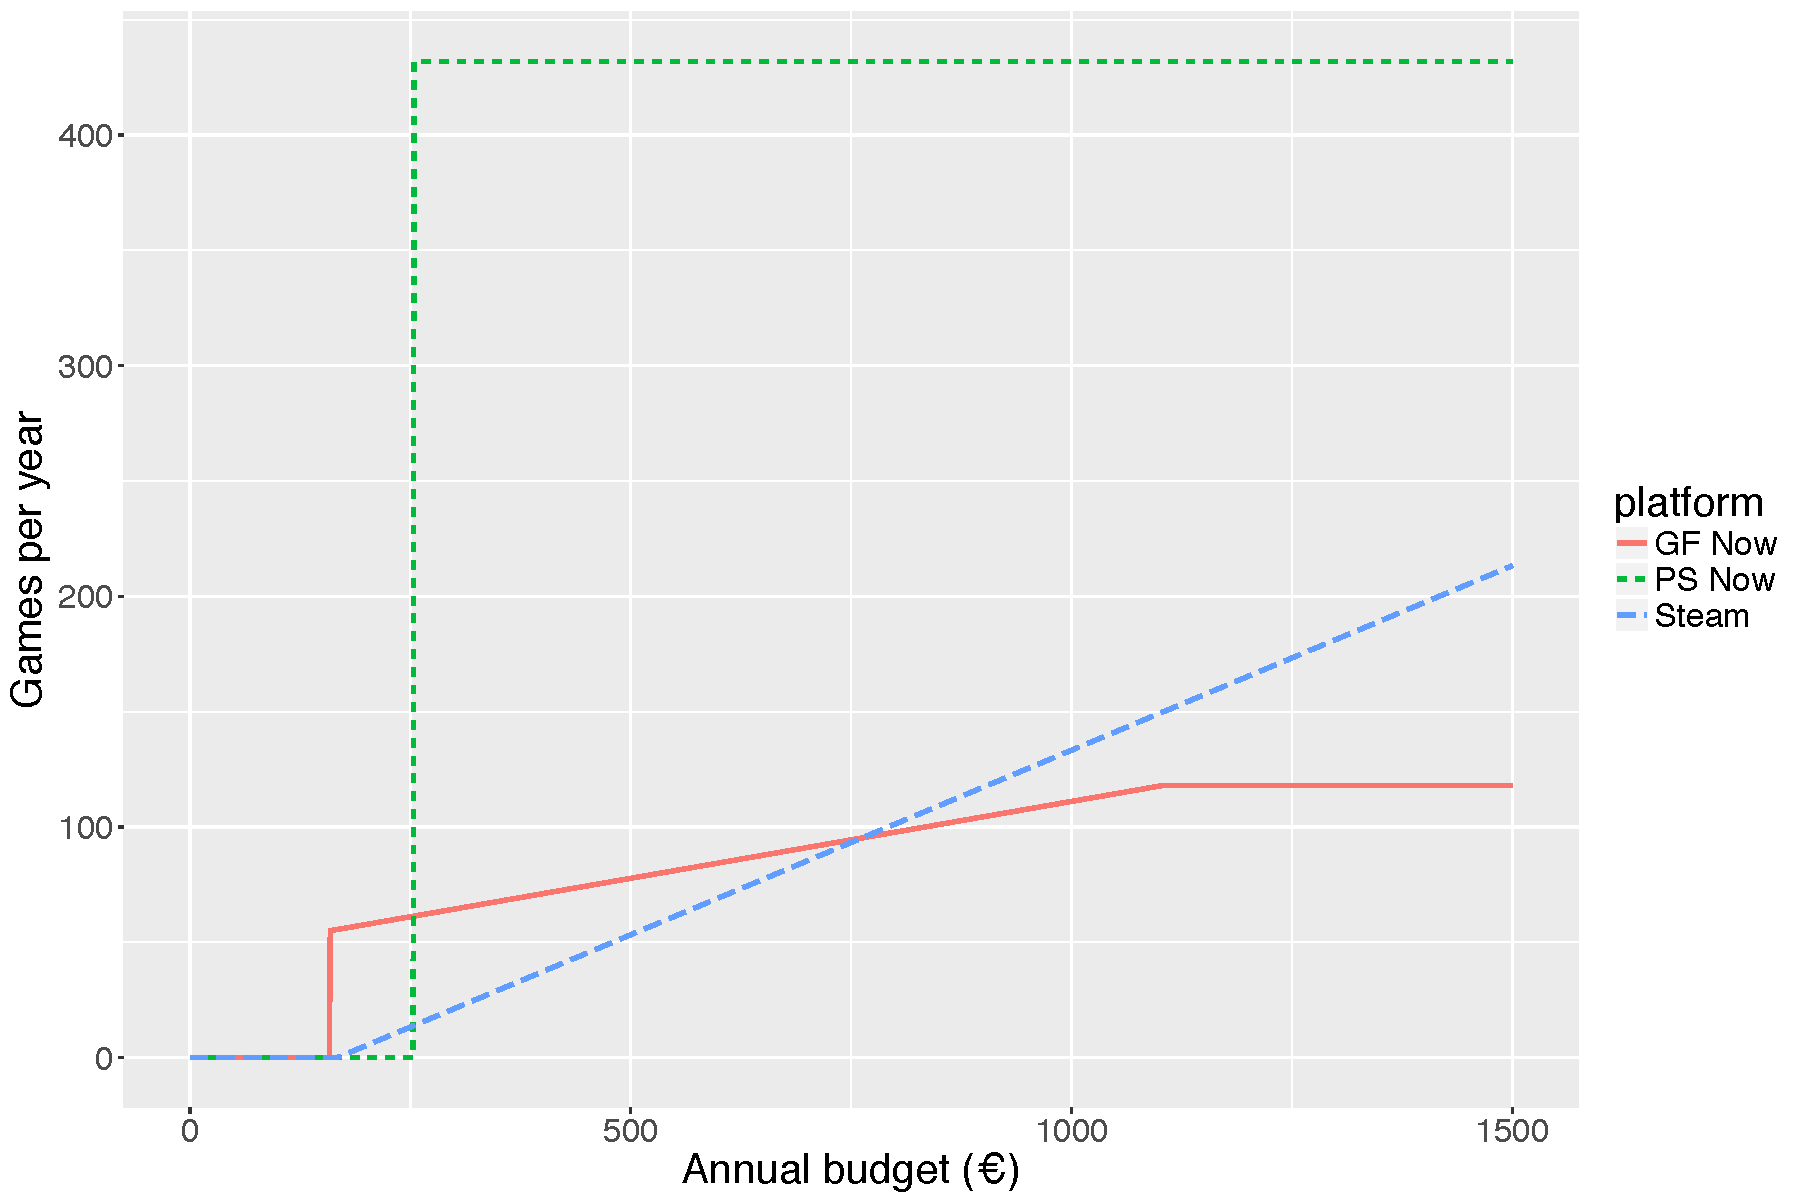
\includegraphics[width=1.0\columnwidth]{images/gamesperyear-over-budget.pdf}
	\caption{Models for several platforms showing the number of games per year that can be bought with a specific \$ budget.}
\label{fig:gamesperyear-over-budget}
\end{figure}

\begin{figure}[!t]
	\centering
	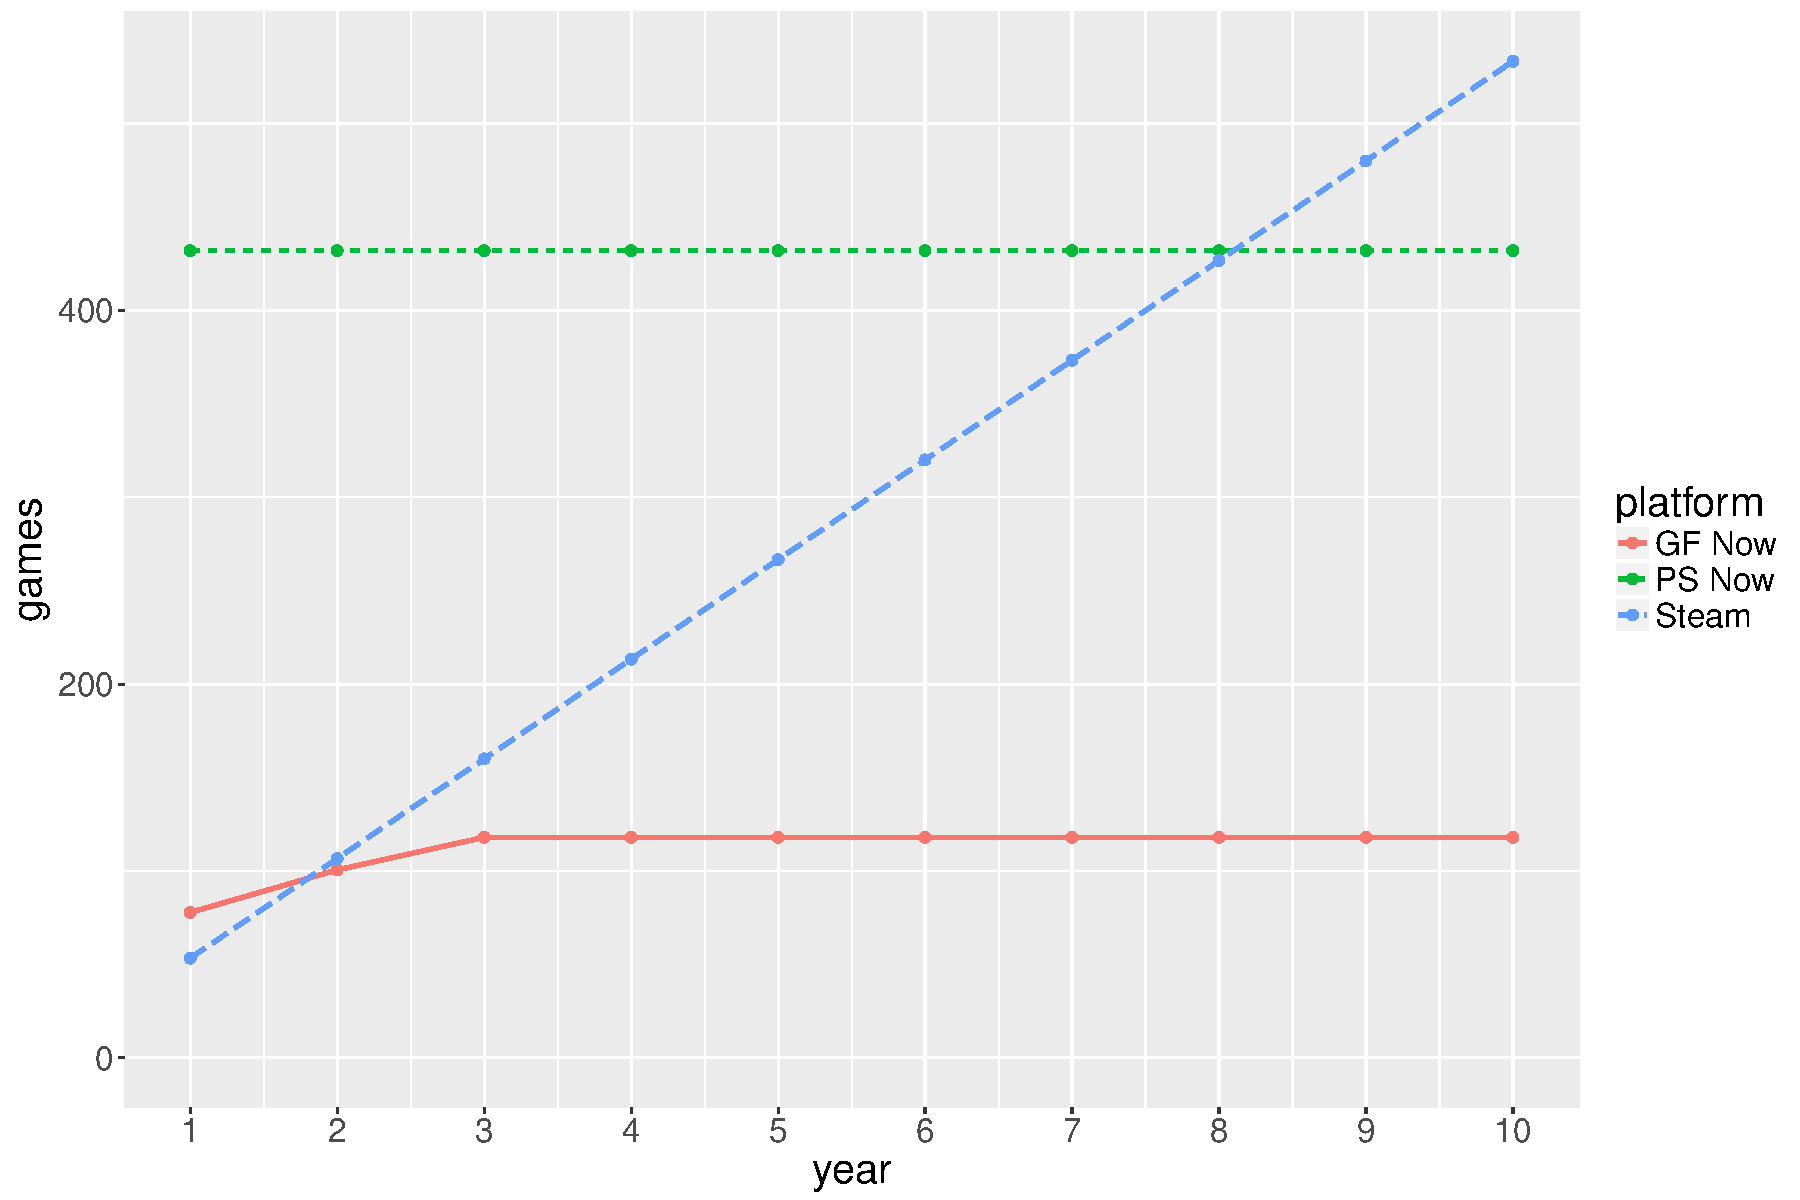
\includegraphics[width=1.0\columnwidth]{images/games-over-year.pdf}
	\caption{Models for several platforms showing the number of games that can be bought over the years subscribed to / using this service.}
\label{fig:games-over-years}
\end{figure}


\subsection{E2E Lag}
End-to-End Lag Model and Simulation in R. Now a standalone (submitted) paper at \url{https://github.com/mas-ude/onlinegame-lag-sim}. Can be referenced to argue the need for low E2E lag (meaning low network delay, but also the need for high fps).


%%%%%%%%%%%%
\subsection{Other Useful Data for Model Creation}

\begin{itemize}
	\item Game costs (current cost possible via Steam dataset; historic price data more difficult)
	\item Length of games (either via howlongtobeat dataset (via \url{https://github.com/mas-ude/gamelengths-scraper}), SteamSpy data, or could also additionally manually parse more Steam data)
	\item Gaming score/ratings/rankings (via Metacritic dataset (via \url{https://github.com/mas-ude/metacritic_scraper}), or might want to additionally scrape steam user review scores)
	\item Other popularity measures? (e.g. steamspy owner data?)
	\item Influence of E2E lag on games? (could be theorized indirectly through e2e lag sim + categorization attempts)
	\item Hardware requirements of games?

	\item Price History? Maybe using steamdb.info?
\end{itemize}

\subsection{Input by Svenja}

After having had a closer look at the merged dataset, several possible relationships between metrics emerge. The success of a game in this case was associated with the ownership, so the more people own a game, the more successful it is.

First of all a few correlation coefficients:
\begin{itemize}
	\item Metacritic score + ownership: 0.2174691 --> This indicates a small effect.
	\item Metacritic user score + ownership: 0.1000701 --> This indicates a small effect, but somehow smaller than the correlation above.
	\item Game length (combined length) + ownership: 0.1767494 --> This indicates a small effect. 
	\item Price + ownership: -0.02796098 --> No effect visible.
\end{itemize}

When plotting the most obvious factors (MC score, length and price) the effects become visually graspable (see figures \ref{fig:rel-score-owners}, \ref{fig:rel-combinedlength-owners} and \ref{fig:rel-price-owners}).

\begin{figure}[!t]
	\centering
	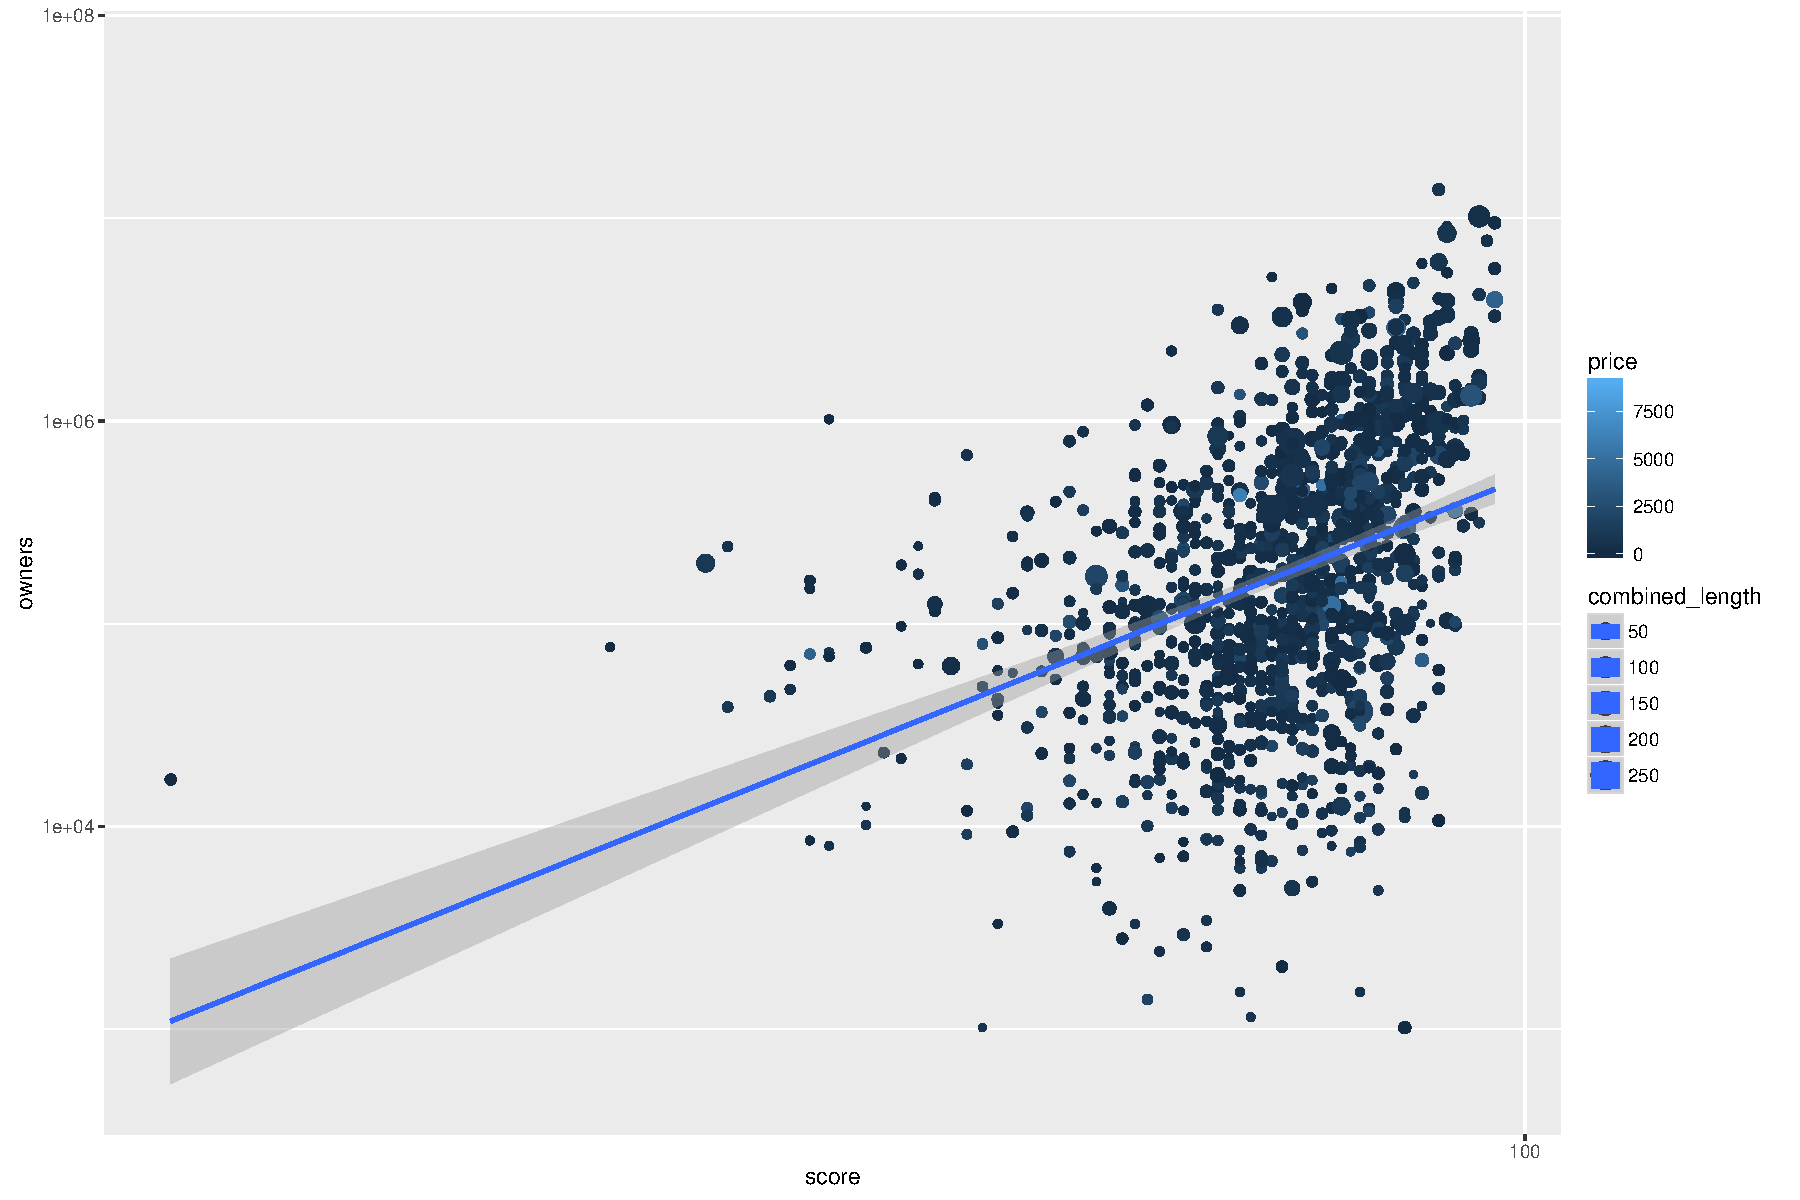
\includegraphics[width=1.0\columnwidth]{images/rel-score-owners.pdf}
	\caption{Relationship Metacritic score to ownership}
\label{fig:rel-score-owners}
\end{figure}

\begin{figure}[!t]
	\centering
	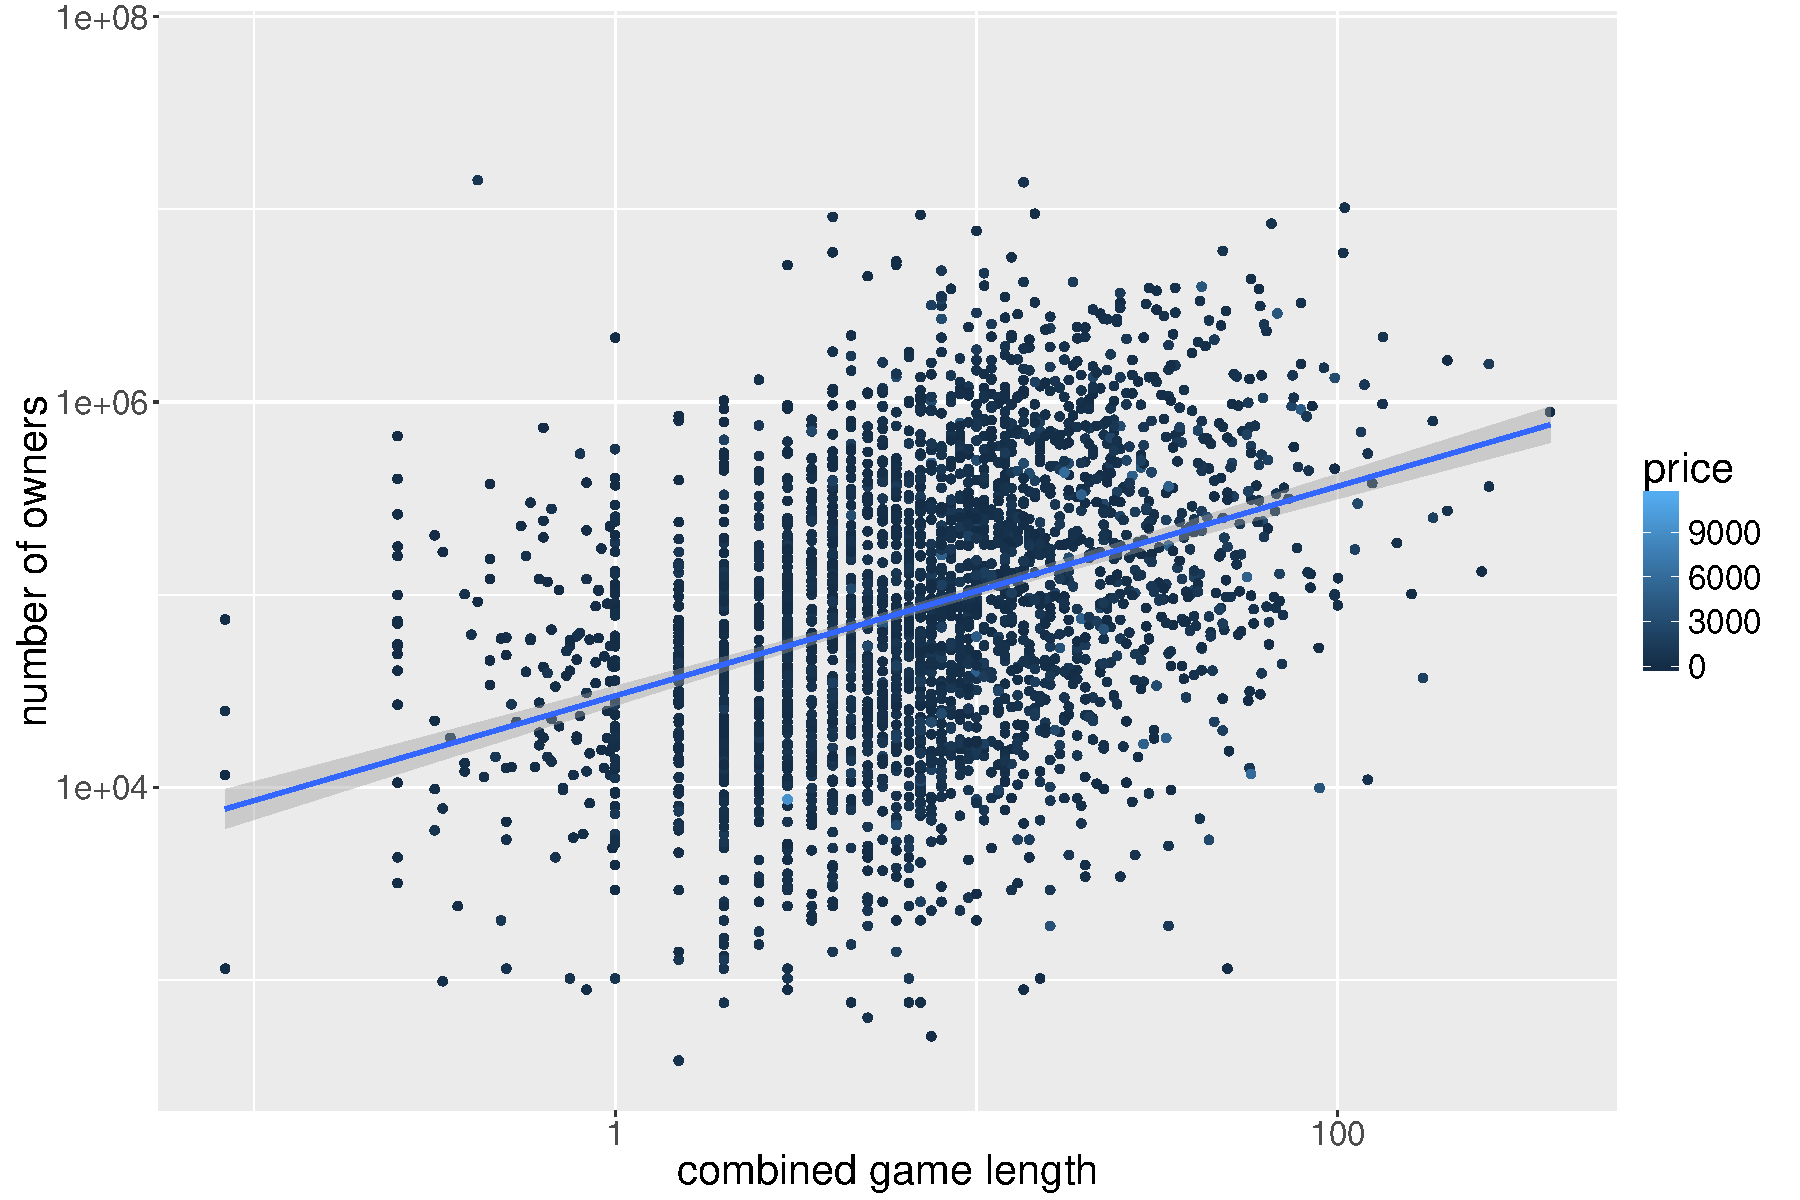
\includegraphics[width=1.0\columnwidth]{images/rel-combinedlength-owners.pdf}
	\caption{Relationship game length to ownership}
\label{fig:rel-combinedlength-owners}
\end{figure}

\begin{figure}[!t]
	\centering
	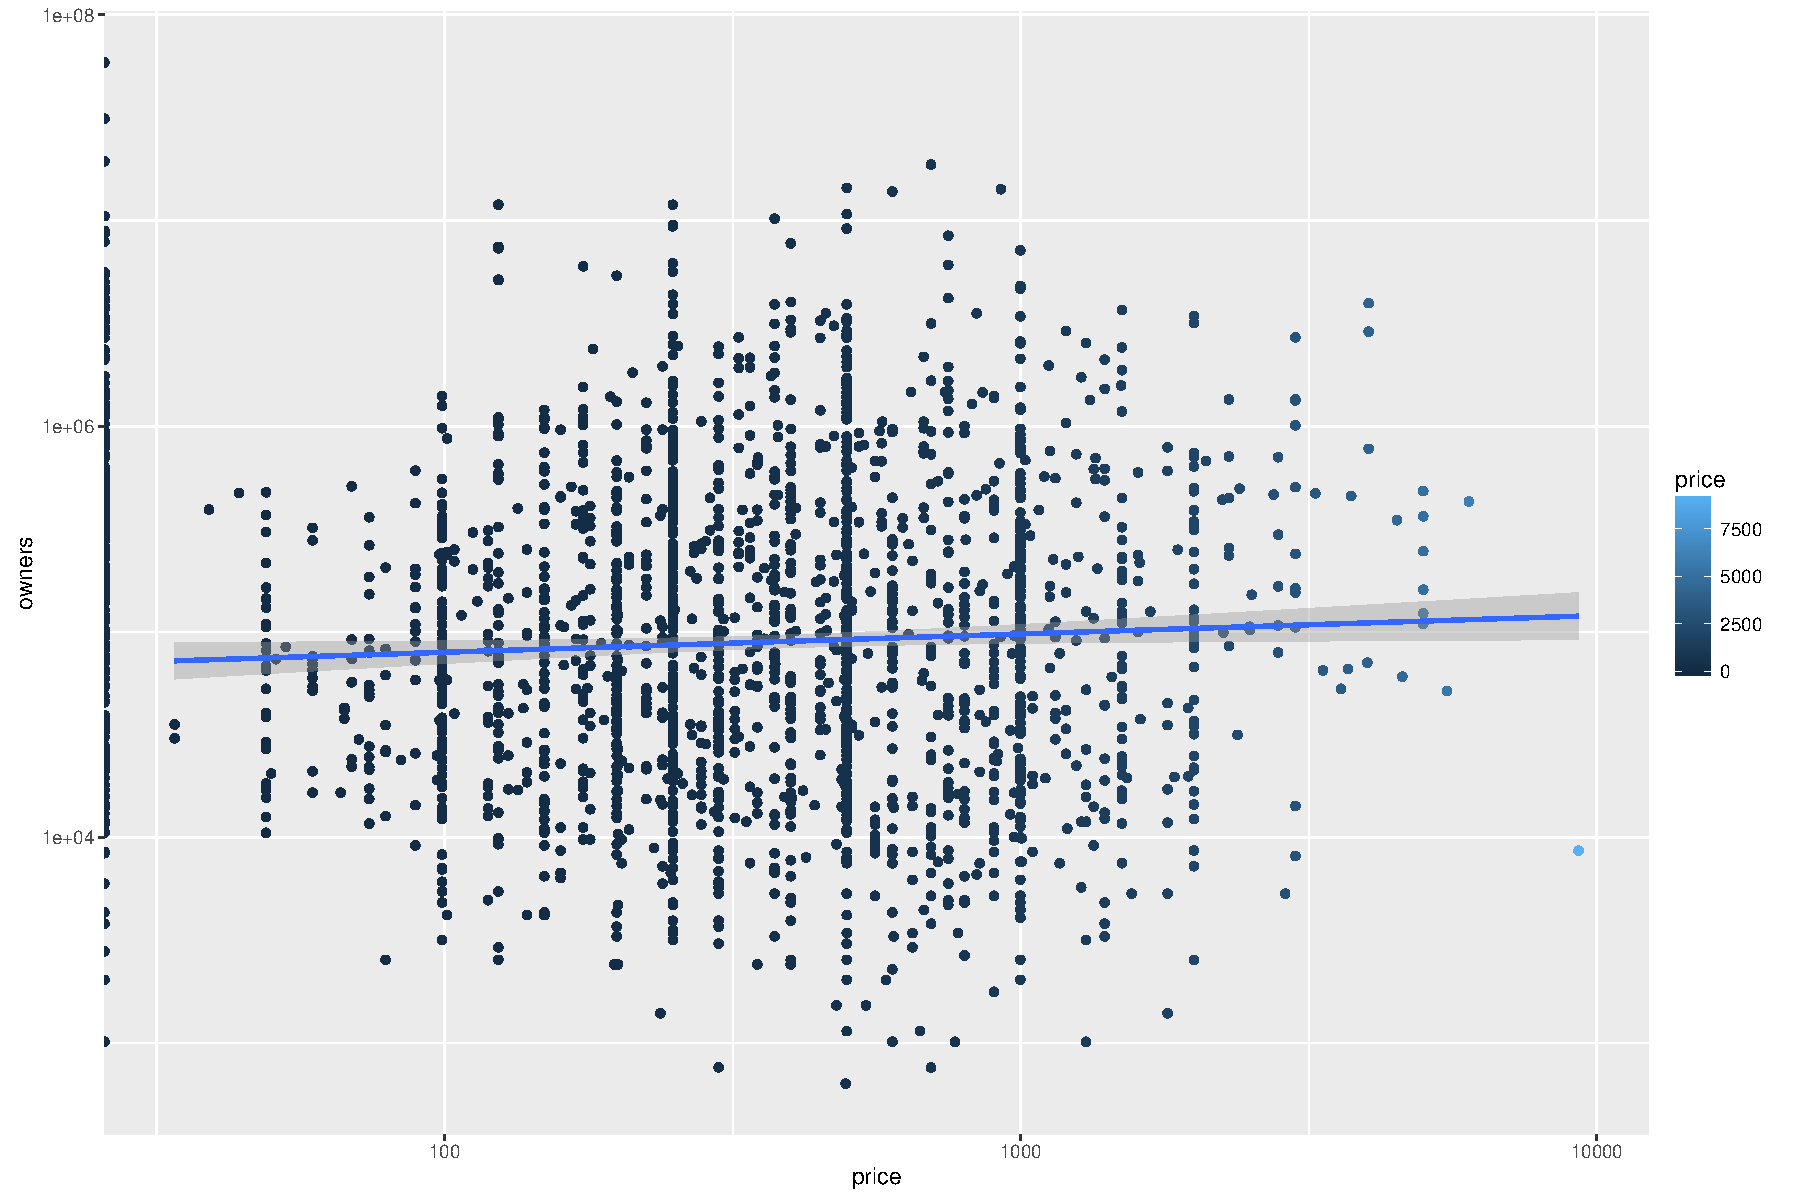
\includegraphics[width=1.0\columnwidth]{images/rel-price-owners.pdf}
	\caption{Relationship price to ownership}
\label{fig:rel-price-owners}
\end{figure}

However, when having a look at figures \ref{fig:rel-price-category-owners} and \ref{fig:rel-score-category-owners}, some details remain unclear: Despite having a relatively low Metacritic score, especially games within the 11-20 range seem to have quite a number of owners - why? Also, either games for free or expensive games seem to be popular. Maybe this is an indicator for the differentiation between hardcore and casual gamers? (Probably it would be interesting as well to track the price over the years and also weigh the ownership count relatively to a game's age.)

\begin{figure}[!t]
	\centering
	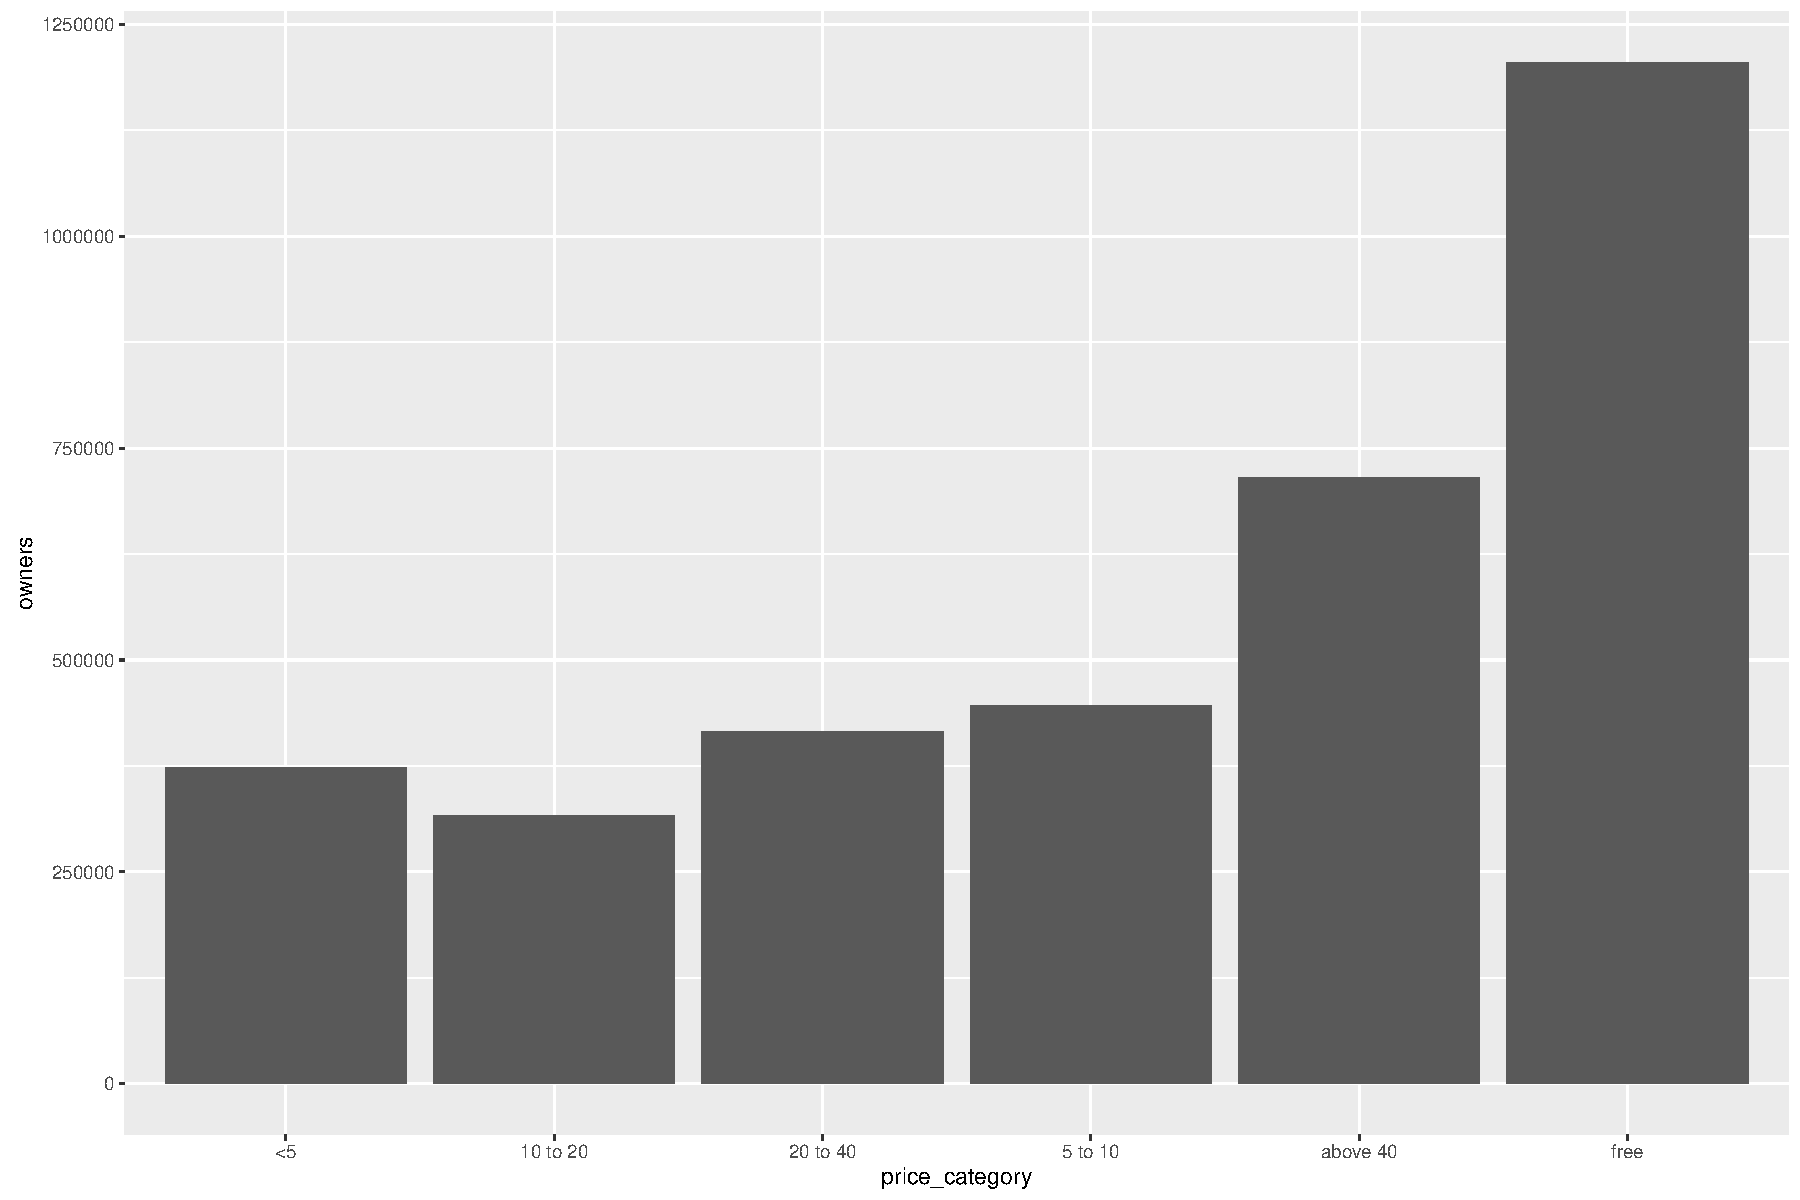
\includegraphics[width=1.0\columnwidth]{images/rel-price-category-owners.pdf}
	\caption{Relationship price category to ownership (\textbf{TODO: Bars need sorting})}
\label{fig:rel-price-category-owners}
\end{figure}

\begin{figure}[!t]
	\centering
	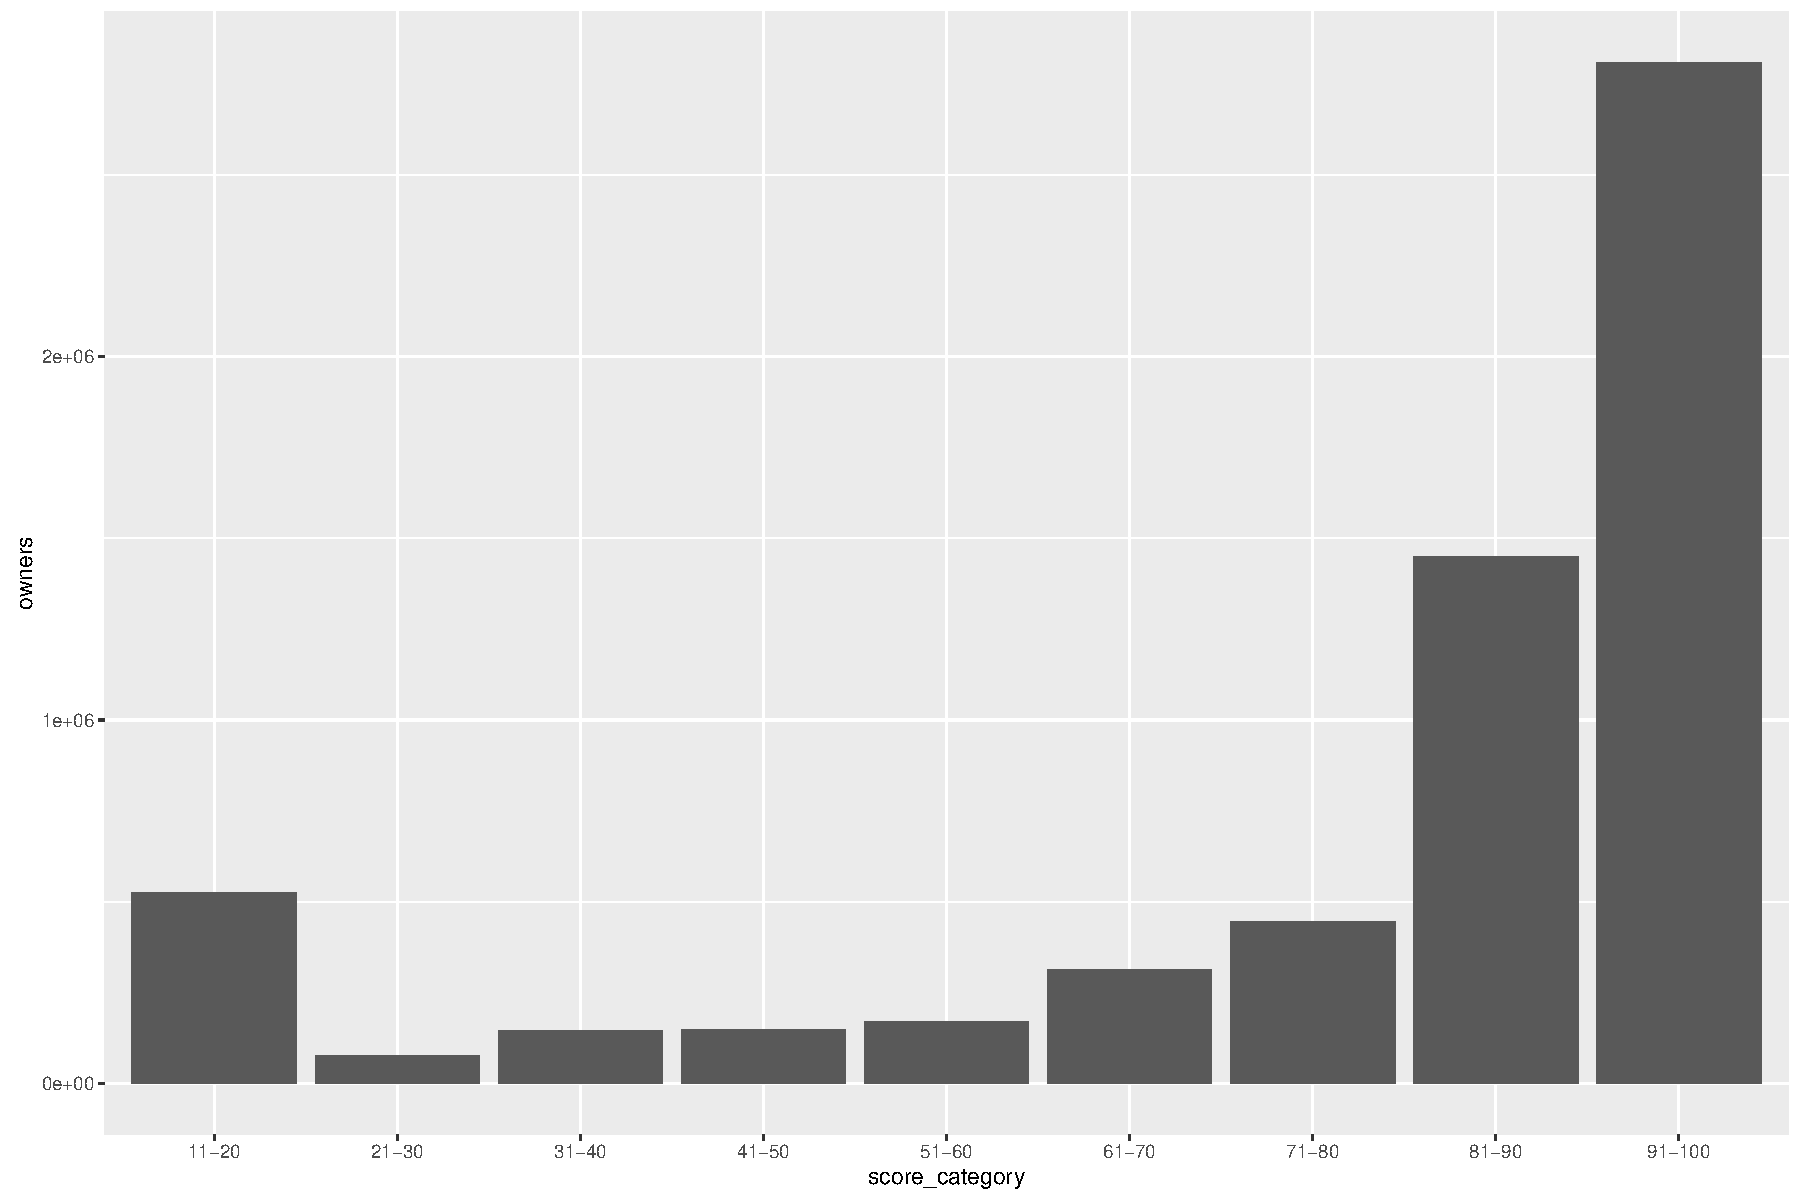
\includegraphics[width=1.0\columnwidth]{images/rel-score-category-owners.pdf}
	\caption{Relationship score category to ownership (\textbf{TODO: Bars need sorting})}
\label{fig:rel-score-category-owners}
\end{figure}

